\documentclass{beamer}
\usepackage{minted}
\usepackage{amsmath,amssymb}
\usepackage{mathtools}
\newcommand{\defeq}{\vcentcolon=}
\newcommand{\eqdef}{=\vcentcolon}
\newcommand{\R}{\mathbb{R}}
\newcommand{\CR}{\hat a^\dagger}
\newcommand{\AN}{\hat a}
\newcommand{\ham}{\hat{\mathcal{H}}}
\newcommand{\Sum}{\sum\limits}
\newcommand{\NO}{\vcentcolon}
\newcommand{\eqsec}{\overset{\CircledTop{2}}{=}}

\AtBeginSection[]
{
    \begin{frame}[plain,noframenumbering]
        \frametitle{Überblick}
        \tableofcontents[currentsection]
    \end{frame}
}
\usemintedstyle{tango}
\usetheme{simple}
%\usepackage{emoji}
\usepackage{lmodern}
\usepackage[scale=2]{ccicons}

% TODO: 
%   position adjustement
%   change colours
%       

% Watermark background (simple theme)

\setwatermark{
\includegraphics[height=8cm]{siegel_watermark.png}}


\title{Flow Equation Approach\\ for Bosonic Impurity Problems}
\subtitle{}
\date{17. Juli 2023}
\author{Jan-Philipp Christ}
\institute{LMU München}

\begin{document}

\maketitle

\begin{frame}{Überblick}
\tableofcontents
\end{frame}


\section{Problemstellung}
\begin{frame}{Problemstellung}
Wie bosonischen Hamiltonian der Form
$$
\hat{\mathcal H} = \underbrace{\sum\limits_k\omega_k\hat a_k^\dagger\hat a_k}_{\eqdef \hat{\mathcal H}_0}+\underbrace{\sum\limits_{q\neq q^\prime}V_{q,q^\prime}\hat a_q^\dagger\hat a_{q^\prime}+\sum\limits_{p,p^\prime}\left( W_{p,p^\prime}\hat a_p^\dagger\hat a^\dagger_{p^\prime}+W_{p,p^\prime}^*\hat a_p\hat a_{p^\prime}\right)}_{\eqdef \hat{\mathcal H}_{\mathrm{int}}}
$$ 
diagonalisieren?

\begin{itemize}
\item bei skalaren Matrix-Elementen eigentlich uninteressant, da auch exakt diagonalisierbar (später)
\item spannender: Matrix-Elemente sind Funktionale der (bosonischen) Besetzungszahlen $\left\{\hat n_k \right\}_k$
\end{itemize}
\end{frame}
\section{Der Flow Equation Approach}
\begin{frame}{Der Flow Equation Approach}
\begin{itemize}
\item Hamiltonian $\ham = \ham_0+\ham_{\mathrm{int}}$
\item Kochrezept zum Herleiten der Gleichungen:
\begin{enumerate}
\item Berechne kanonischen Generator $\hat\eta=\left[\ham_0,\ham_{\mathrm{int}}\right]$
\item Berechne $\left[\hat\eta,\ham\right]$ \\
$\rightarrow$ Terme der Form $\left(\prod\limits_{k_i}\CR_{k_i}\right)\cdot\left(\prod\limits_{\kappa_i}\AN_{\kappa_i}\right)$ werden mit $\left(\Sum_{k_i}\omega_{k_i}-\Sum_{\kappa_i}\omega_{\kappa_i}\right)^2$ multipliziert
\item Schließe auf Form des Flow Hamiltonians. Wenn Flow Hamiltonian nicht von gleicher Form wie ursprünglicher Hamiltonian, gehe zu 2.
\item Flow Equations durch Koeffizientenvergleich in $$\frac{\mathrm d\ham(\lambda)}{\mathrm d\lambda} = \left[\hat\eta(\lambda),\ham(\lambda)\right]$$
\end{enumerate}
\end{itemize}
\end{frame}
\section{Flow Equations im rein quadratischen Fall}
\begin{frame}{Flow Equations im rein quadratischen Fall}
\includegraphics[scale=.7]{Feq.png}
\end{frame}
\section{Implementierung des rein quadratischen Falls}
\begin{frame}[fragile]

\frametitle{Main}

\begin{minted}[breaklines,fontsize=\scriptsize]{Julia}
flat = npzread(PATH*name)
om0,V0,W0,eps0 = unpack_arr(flat,N)
om0 = om0 + diag(V0)        
V0 = V0 - Diagonal(diag(V0))
        
u0 = flat_arr(om0,V0,W0,eps0)

tspan = (0.0,30)

prob = ODEProblem(f,u0,tspan,[N])
sol = solve(prob, Tsit5(),saveat=LinRange(tspan[1],tspan[2],n), reltol = 1e-8, abstol = 1e-8)
        
npzwrite(SAVEPATH*FILENAME,sol)
npzwrite(SAVEPATH*"sol_full_t"*name,sol.t)
\end{minted}

$$\rightarrow\ \text{sehr langsam :-(}$$

\vfill
ABER$\ldots$ einige Verbesserungen denkbar und möglich

\end{frame}
\begin{frame}[fragile]

\frametitle{Hilfsfunktionen}

\begin{minted}{Julia}
using NPZ, DifferentialEquations, LinearAlgebra

function flat_arr(om,V,W,eps)
    return vcat(vec(om),vec(V),vec(W),eps)
end

function unpack_arr(flat,N)
    N = Int(N)
    om0 = flat[1:N]
    V0 = flat[N+1:N+Int(N^2)]
    W0 = flat[N+Int(N^2)+1:N+Int(2*N^2)]
    eps = flat[end]
    V = reshape(V0,(N,N))
    W = reshape(W0,(N,N))
    return om0,V,W,eps
end
\end{minted}

\end{frame}

\begin{frame}[fragile]

\frametitle{Definition der ODE}

\begin{minted}[breaklines,fontsize=\scriptsize]{Julia}
function f(u,p,t)
    N = Int(p[1]); om,V,W,eps = unpack_arr(u,N); Wdag = conj(W)

    om_ret = [sum([2*V[q,k]*V[k,q]*(om[k]-om[q]) -2*(W[k,q]+W[q,k])*(om[k]+om[q])*(Wdag[q,k]+Wdag[k,q]) for q in 1:N]) for k in 1:N]

    V_ret = reshape([-V[q,q_]*(om[q]-om[q_])^2 +sum([-(W[(q),p]+W[p,(q)])*(Wdag[p,(q_)]+Wdag[(q_),p])*(om[(q)]+om[(q_)] +2*om[p])+V[p,(q_)]*V[(q),p]*(om[(q)]+om[(q_)] -2*om[p]) for p in 1:N]) for q_ in 1:N for q in 1:N],(N,N)).*(ones(N,N)-Diagonal(ones(N)))

    W_ret = reshape([-W[p,p_]*(om[p]+om[p_])^2 +sum([-V[p,q]*(om[q]+om[p_])*(W[p_,q]+W[q,p_]) +V[p,q]*(om[p]-om[q])*(W[q,p_]+W[p_,q]) for q in 1:N]) for p_ in 1:N for p in 1:N],(N,N))

    eps_ret = -2*sum([(W[p,p_]+W[p_,p])*(om[p]+om[p_])*Wdag[p,p_] for p in 1:N for p_ in 1:N])

    return flat_arr(om_ret,V_ret,W_ret,eps_ret) 
end
\end{minted}


\end{frame}

\section{Der physikalische Rahmen}
\subsection{Das 1D Bose Polaron}
\begin{frame}[allowframebreaks]{Das 1D Bose Polaron}
Fröhlich Hamiltonian:
$$
\ham_F = g_{IB}n_0+\frac{\hat p^2}{2M}+\int\mathrm d k\omega_{ k}\CR_{ k}\AN_{ k}+\sqrt{\frac{n_0}{2\pi}}g_{IB}\int\mathrm d k W_k e^{ik\hat x}\left(\AN_{ k}+\CR_{- k}\right)
$$
Zwei-Phonon Streuung:
$$
\ham_{2\mathrm{ph}}=\frac{g_{IB}}{2\pi}\int\mathrm d k\mathrm d k^\prime \left(c_k\CR_k-s_k\AN_{-k}\right)\left(c_{k^\prime}\AN_{k^\prime}-s_{k^\prime}\CR_{-k^\prime}\right)e^{i(k-k^\prime)x}
$$
Gesamthamiltonian
$$
\ham = \ham_F + \ham_{2\mathrm{ph}}
$$
ist nicht in unserer rein quadratischen Form von vorhin.
\end{frame}
\subsection{Die LLP- und die Displacement Transformation}
\begin{frame}[allowframebreaks]{Die LLP- und die Displacement Transformation}
LLP-Transformation: Nutze Erhaltung des \emph{Gesamt}impulses, um in mit der Impurity bewegtes Bezugssystem zu transformieren
$$
\hat U_{\mathrm{LLP}}\defeq \exp\left(i\hat x\cdot \hat p_b\right)
$$
Hamiltonian ist dann:
\begin{align*}
\hat U_{\mathrm{LLP}}^\dagger\ham\hat U_{\mathrm{LLP}} &\defeq \ham_{\mathrm{LLP}}(p) =g_{IB}n_0+\frac{1}{2M}\left(p-\int\mathrm d k k \CR_k\AN_k \right)^2\\ &+\int\mathrm d k\omega_{ k}\CR_{ k}\AN_{ k}+\sqrt{\frac{n_0}{2\pi}}g_{IB}\int \mathrm d k W_k \left(\AN_{ k}+\CR_{- k}\right) \\ &+ \frac{g_{IB}}{2\pi}\int\mathrm d k\mathrm d k^\prime \left(c_k\CR_k-s_k\AN_{-k}\right)\left(c_{k^\prime}\AN_{k^\prime}-s_{k^\prime}\CR_{-k^\prime}\right)
\end{align*}
\vfill
\framebreak
Displacement Transformation:
$$
\hat D(\underline\alpha)\defeq\exp\left(\sum_k\alpha_k\CR_k-\mathrm{h.c.}\right)=\exp\left(-\underline\alpha^\dagger{\underline{\underline\Omega}}\ \underline{\hat a}\right)
$$
Wirkung auf Erzeugungs- und Vernichtungsoperatoren:
\begin{align*}
\hat D^\dagger(\underline \alpha)\AN_{k_i}\hat D(\underline\alpha)&=\AN_{k_i}+\alpha_{k_i}\\
\hat D^\dagger(\underline \alpha)\CR_{k_i}\hat D(\underline\alpha)&=\CR_{k_i}+\alpha_{k_i}^*
\end{align*}
$$
\rightarrow \text{transformiere lineare Terme weg durch geeignete Wahl von}\ \underline\alpha
$$
\end{frame}

\section{Ergebnisse- was haben wir gelernt?}
\begin{frame}[allowframebreaks]{Ergebnisse- was haben wir gelernt?}
\begin{itemize}
\item anfängliche Symmetrie $k\leftrightarrow-k$ des Hamiltonians verhindert Konvergenz der Flow Equations zum exakten Spektrum\\
$\rightarrow$ führe twisted boundary conditions ein
\end{itemize}
\begin{figure}[H]
    \centering
    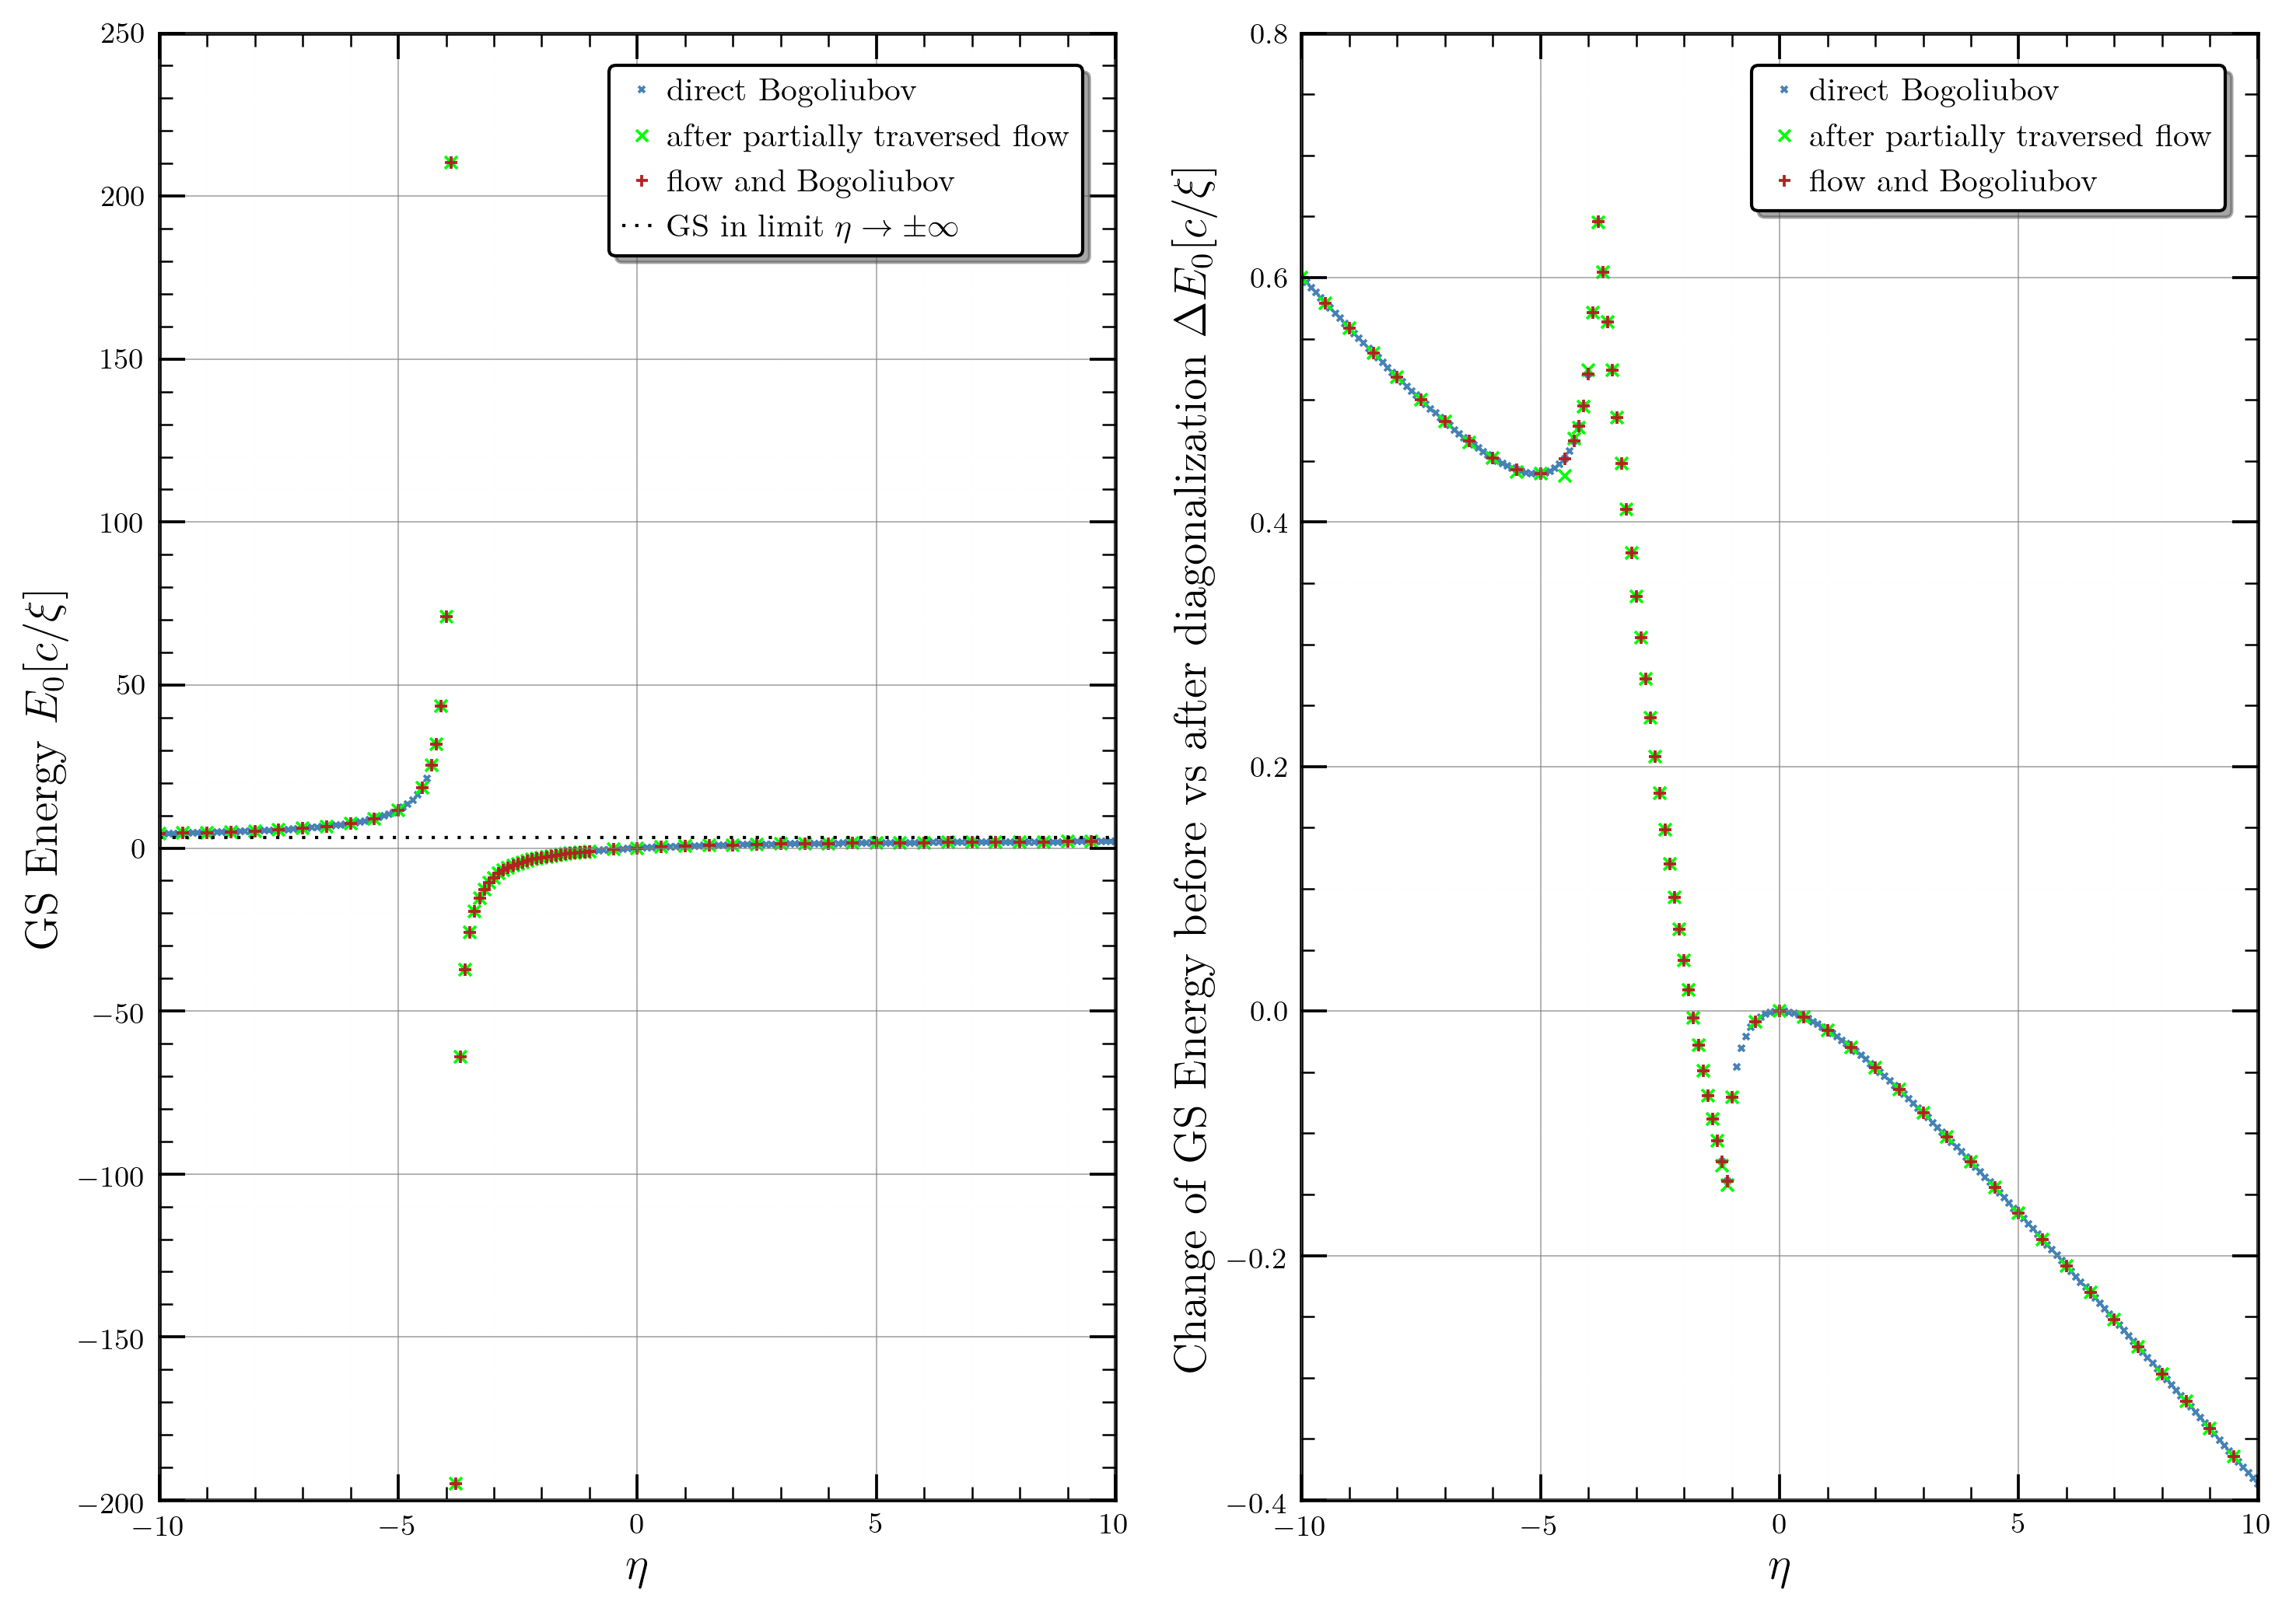
\includegraphics[scale=0.35]{figures/plots/PNG/GS_energies_bog_flow_comp_N=40.png}
\end{figure}
\framebreak
\begin{itemize}
\item Verschiebung des $k-$grids bricht Symmetrie, Konvergenz zum exakten Spektrum des Hamiltonian wird erreicht
\begin{figure}[H]
    \centering
    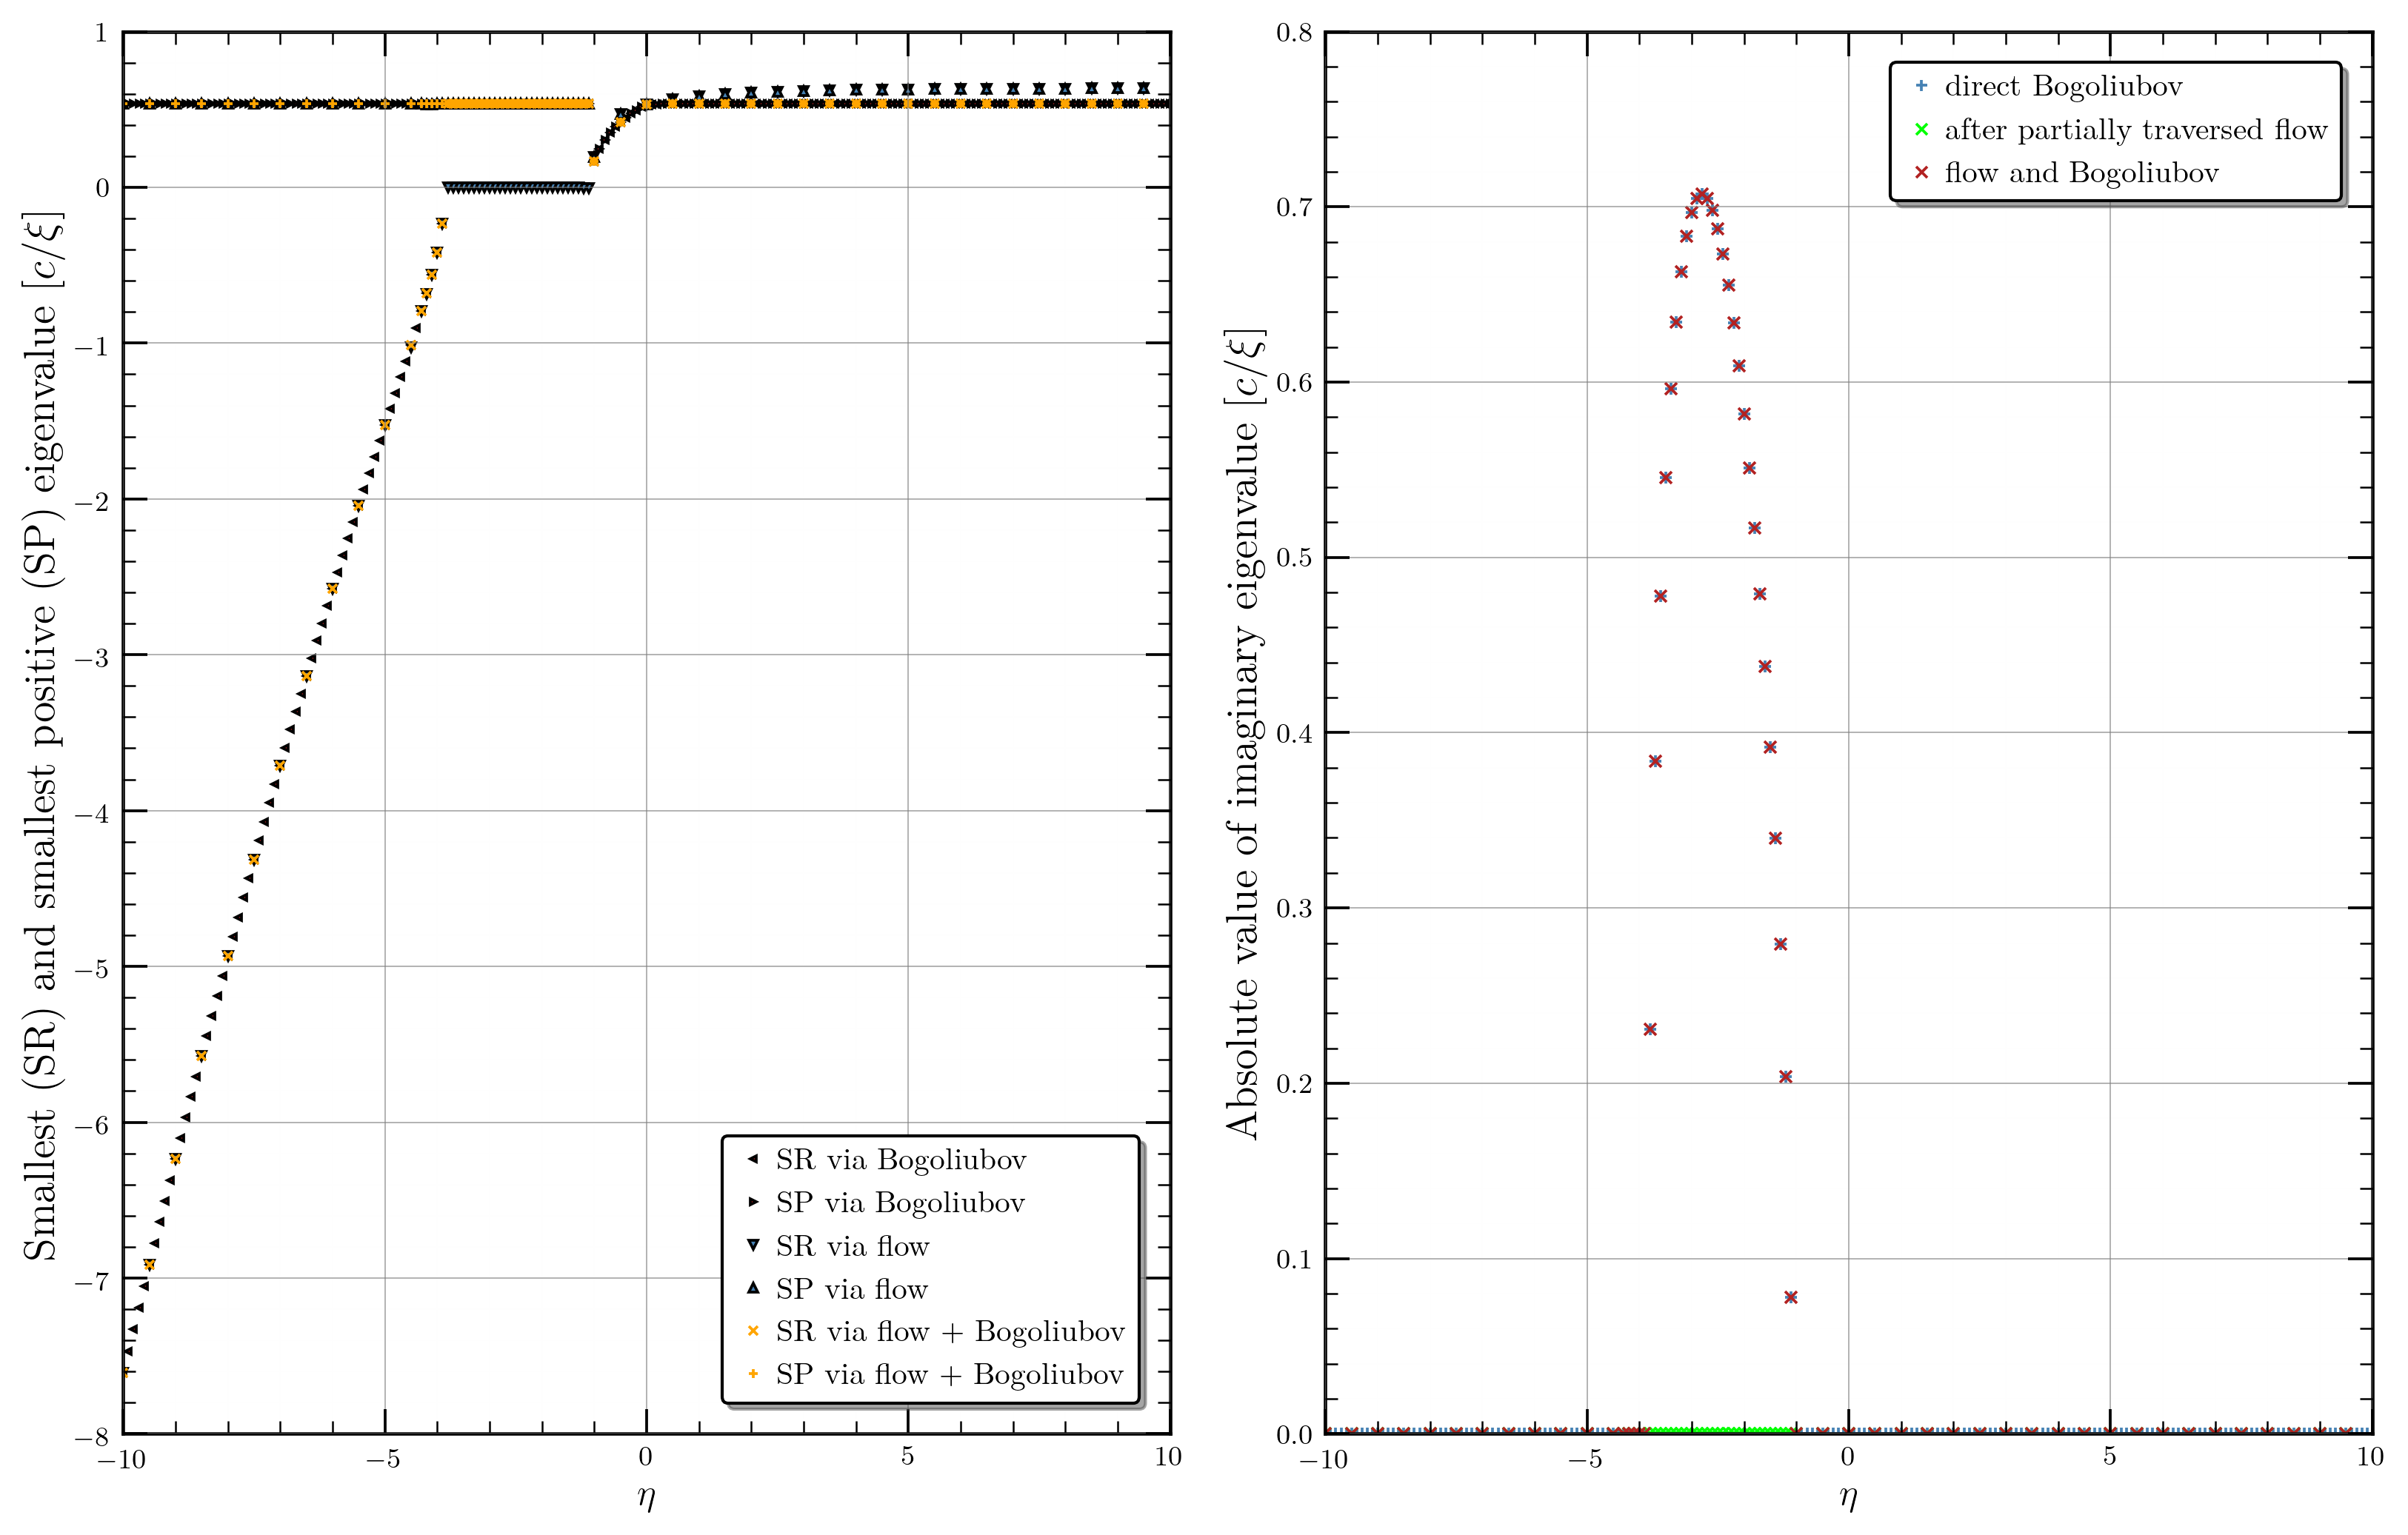
\includegraphics[scale=0.35]{figures/plots/PNG/spectrum_analysis_bog_flow_comp_N=40.png}
\end{figure}
\end{itemize}
\end{frame}
\section{Was kommt jetzt? - Ausblick}
\begin{frame}{Was kommt jetzt? - Ausblick}
a
\end{frame}

\begin{frame}
\begin{centering}
Und nun her mit den Fragen :-)
\end{centering}
\end{frame}
\end{document}
